%----------------------------
% CHAPTER 8: System Analysis
%----------------------------

\chapter{System Analysis}

\label{chapter08}

Once the whole application is finished, here is an evalution. Lets see if it satisfies all functional requirements and show some examples of usage.

\section{Requirements satisfaction}

All functional requirements except eight must be satisfied in the Web UI. The last is satisfied by the Comparison Service. Let's review them and explain how they all get satisfied:

\begin{enumerate}
    \item \textbf{Search availability values by origin, destination, month and year}: \textit{Let the user of the \thesis\ search available flights evolution by date, for a given route (origin and destination), month and year of the flight.}
    \\\\
    In the search component, the user can select available flights, set an origin, destination, month and year.
    \begin{figure}[H]
    \centering
    
\includegraphics[scale=0.35]{resources/search-availability.png}
    \caption{Demo of the search available flights functionality.}
    \end{figure}

    \item \textbf{Search searches values by origin, destination, month and year}: \textit{Same as feature \#1, but for user searches instead of available flights.}
    \\\\
    In the search component, the user can select user searches, set an origin, destination, month and year.
    \begin{figure}[H]
    \centering
    
\includegraphics[scale=0.35]{resources/search-searches.png}
    \caption{Demo of the search user searches functionality.}
    \end{figure}

    \item \textbf{Search multiple availability values}: \textit{Be able to search and show multiple availability values for different flights in the same chart, easing the comparison between both queries. For example: Route A-B in August 2018 shows more availability than route A-C in August 2018 from January to March, but A-C has more availability than A-B from April until today.}
    \\\\
    Once the user has searched for flight availability, it can search again and the results will appear in the chart.
    \begin{figure}[H]
    \centering
    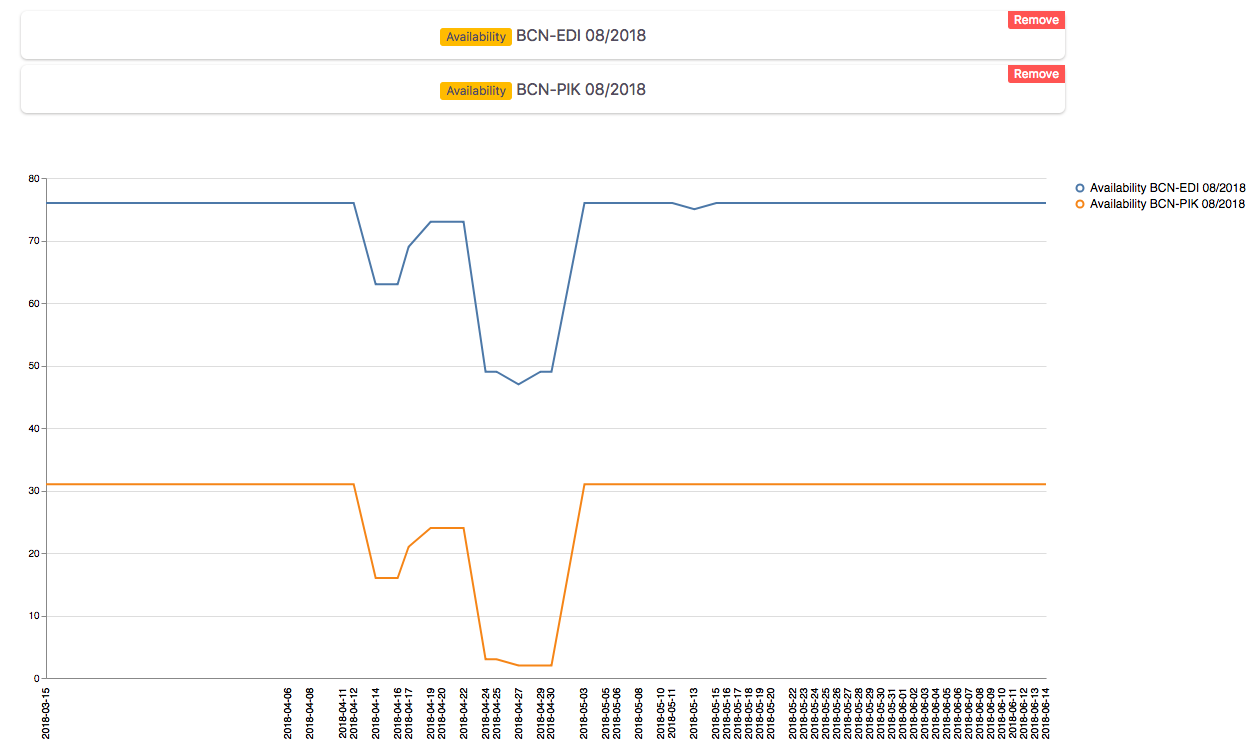
\includegraphics[scale=0.3]{resources/search-multiple-availability.png}
    \caption{Demo of the search multiple available flights functionality.}
    \end{figure}

    \item \textbf{Search multiple searches values}: \textit{Be able to query and display multiple user searches values for different routes in the same chart, easing the comparison between both queries. For example: Route A-B in August 2017 shows more searches than route A-B in December 2017 from January to June.}
    \\\\
    Once the user has searched for user searches, it can search again and the results will appear in the chart.
    \begin{figure}[H]
    \centering
    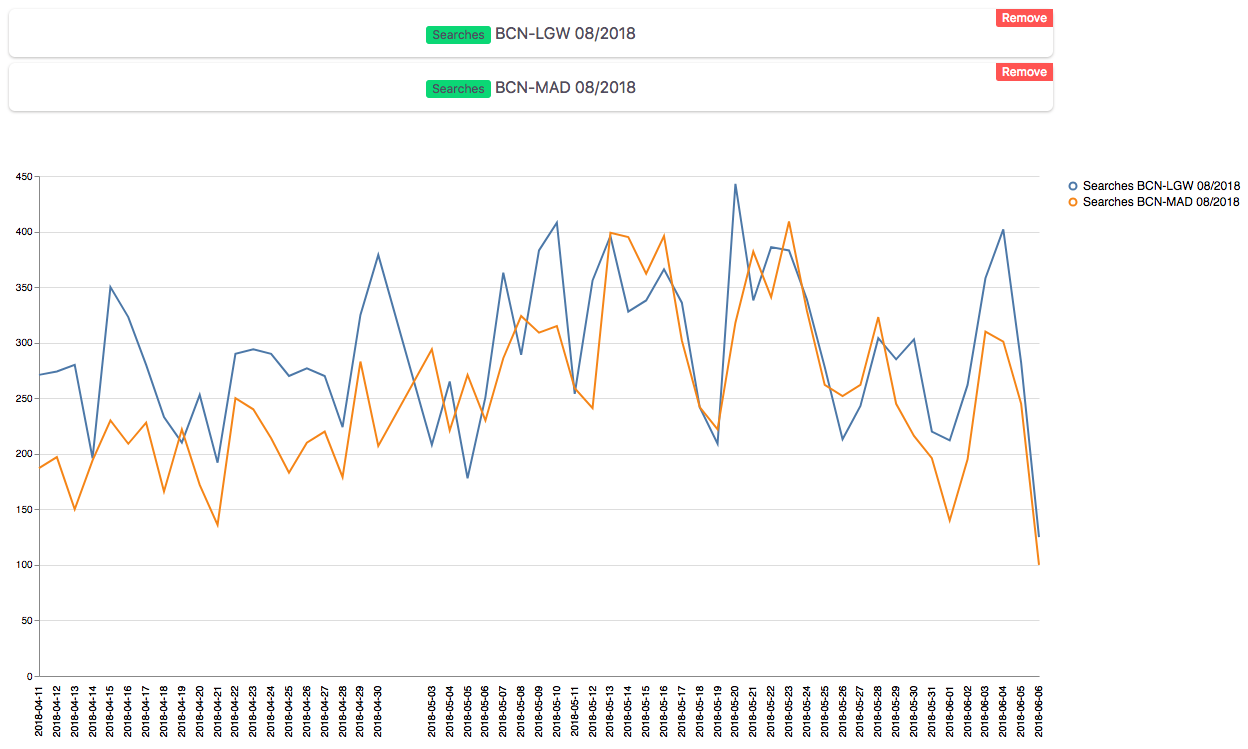
\includegraphics[scale=0.3]{resources/search-multiple-searches.png}
    \caption{Demo of the search multiple user searches functionality.}
    \end{figure}

    \item \textbf{Search multiple mixed values}: \textit{Enable comparison between availability and searches as well. Search and display the comparison in the chart.}
    \\\\
    In the search component, the user can select the comparison field, set an origin, destination, month and year. It is the same as search first for available flights and then for user searches with the same parameters.
    \begin{figure}[H]
    \centering
    
\includegraphics[scale=0.35]{resources/search-comparison.png}
    \caption{Demo of the search comparison functionality.}
    \end{figure}

    \item \textbf{Add new query to chart}: \textit{Search for offer or demand (features \#1 or \#2) and display the result in the chart.}
    \\\\
    Every time the user searches for data, the query is \textbf{added} to the chart.
    \begin{figure}[H]
    \centering
    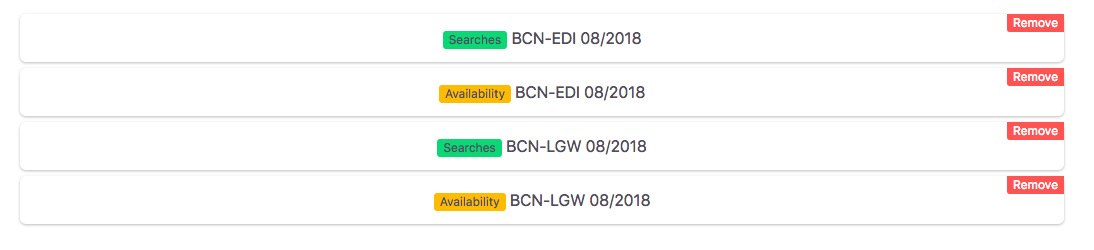
\includegraphics[scale=0.35]{resources/queries-list.png}
    \caption{Demo of the queries functionality.}
    \end{figure}

    \item \textbf{Remove query from chart}: \textit{Remove data from the chart, stop displaying an specific query's data.}
    \\\\
    Each query has a remove button that removes it from the chart.
    \begin{figure}[H]
    \centering
    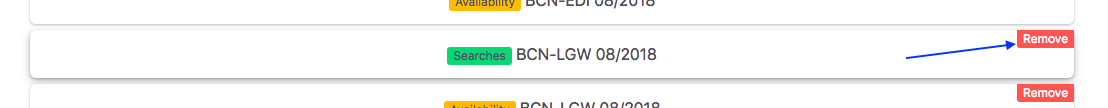
\includegraphics[scale=0.35]{resources/queries-remove.png}
    \caption{Demo of the remove queries functionality.}
    \end{figure}

    \item \textbf{Historical data API}: Enable an endpoint where developers can get historical data for a given route, month, year and source (available flights and user searches).
    \\\\
    \begin{verbatim}
    GET /api/historical/prod/searches/BCN-EDI/2018-10

    RESPONSE
    {
        queries: [
            {
                id: 1529050761587,
                name: "Searches BCN-EDI 10/2018",
                source: "Searches",
                origin: "BCN",
                destination: "EDI",
                month: "10",
                year: "2018"
            }
        ],
        results: [
            {
                date: 1523404800000,
                version: "2018-04-11",
                count: 122,
                key: 1529050761587
            },
            {
                date: 1523491200000,
                version: "2018-04-12",
                count: 197,
                key: 1529050761587
            },
            {
                date: 1523577600000,
                version: "2018-04-13",
                count: 143,
                key: 1529050761587
            },
            ...
        ]
    }
    \end{verbatim}
    In this response, the results object contains an array of records, each one with the date in milliseconds, the date in human format (version), amount of searches or available flights (count), and a key that is the same for all the results and the same as the query. This data has enough detail for the developer start making some analysis.

\end{enumerate}

\section{Data experiment}

Right now the database does not have much data. Is very difficult to extract tendencies, there are only records from the last two months. Even so, there is enough to make some conclusions from the different comparisons.
\\\\
There are some examples of usage of the \thesis.

\subsection*{Experiment 1} \label{exp1}

What London airport people prefer when traveling from Barcelona?
\\\\
There are six airports in London, searching user demand from Barcelona to those airports for traveling in October 2018 we get the following chart:

\begin{figure}[H]
\centering
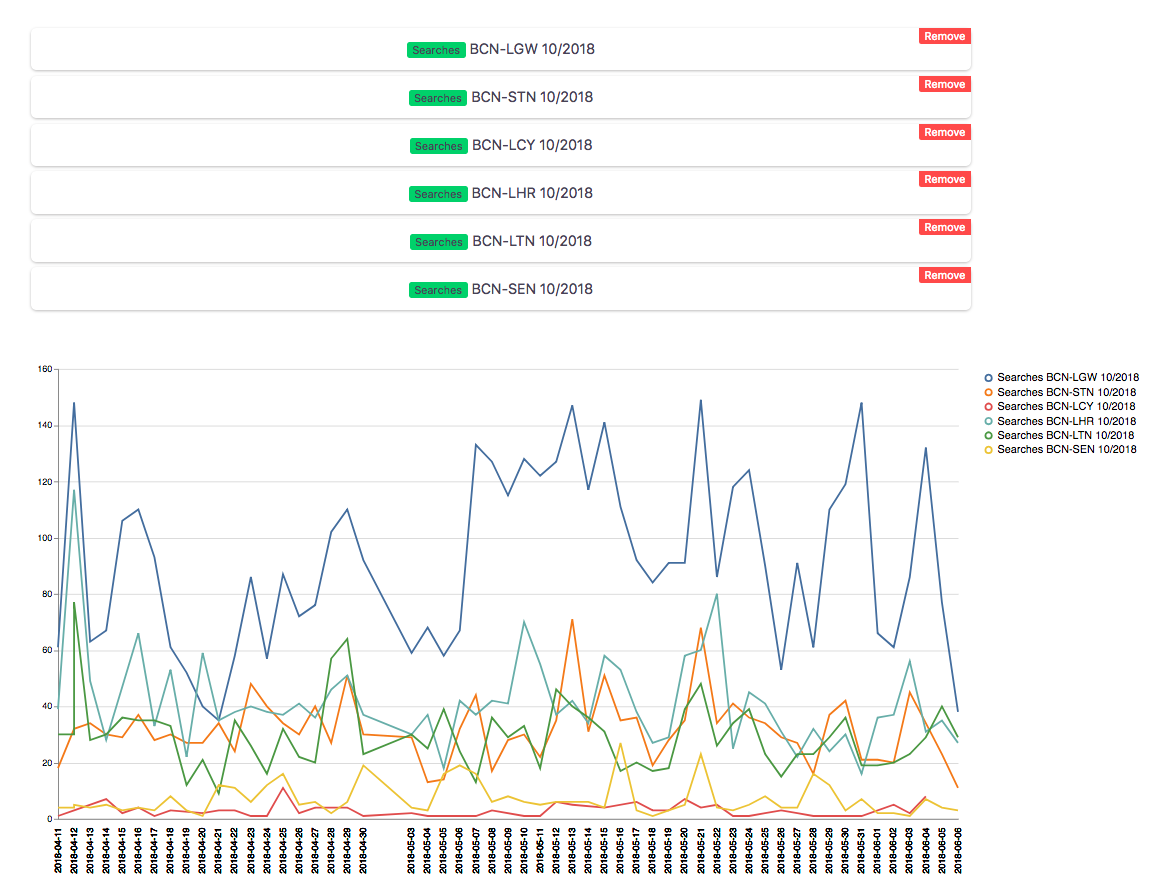
\includegraphics[scale=0.3]{resources/experiment01.png}
\caption{Searches from Barcelona to London Airports October 2018}
\end{figure}

From its six airports: City, Heathrow, Gatwick, Luton, Stansted and Southend; Heathrow is the London Airport with more passengers (78 million in 2017\cite{london_traffic}) but Gatwick (45 million passengers in 2017) is the preferred airport when traveling from Barcelona.

\subsection*{Experiment 2} \label{exp2}

When traveling from New York (JFK), the results are different:

\begin{figure}[H]
\centering
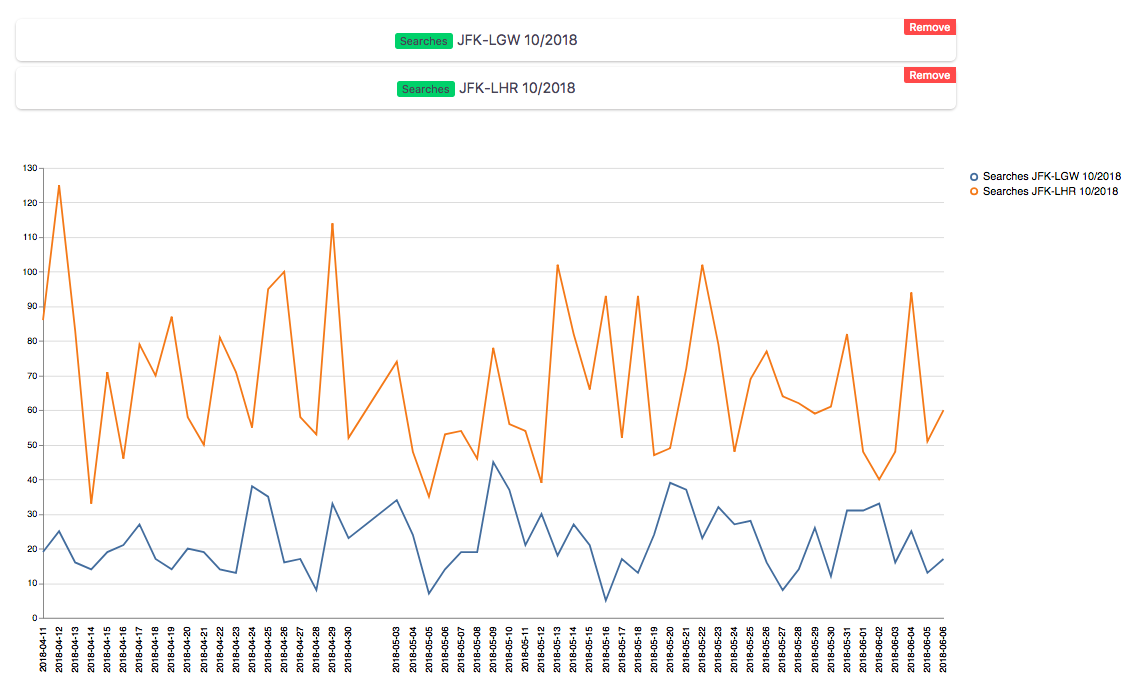
\includegraphics[scale=0.35]{resources/experiment02.png}
\caption{Searches from New York JFK to LHR and LGW October 2018}
\end{figure}

London Heathrow is searched more than London Gatwick. Provably because Heathrow usually operates longer flights than Gatwick airport.

